\begin{activite}[Segments, droites et demi-droites]

 \begin{partie}[À la découverte d'un nouveau code]
  \begin{enumerate}
   \item Lire la consigne de la case \circled{1} et observer la figure correspondant à cette consigne.
Faire de même pour la case \circled{2}.

Quand le code est compris, tracer la figure de la case \circled{3} et écrire la consigne de la case \circled{4}.


  \vspace{1em}
  
  \begin{tabular}{|c|c|c|c|c|}
  \cline{1-2}\cline{4-5}
    \circled{1} 		& \circled{2} 		& 	& \circled{3} 		& \circled{4}	\\ 
     Tracer $(AB)$ 	&  Tracer $[AC)$ 	& 	& Tracer $(AB)$	& 	 		\\ 
     Tracer $[AC]$ 	& Tracer $[BC]$ 	& 	& Tracer$[BC]$		& 			\\
     				&				&	& Tracer$[AC)$		&			\\ \cline{1-2}\cline{4-5}
   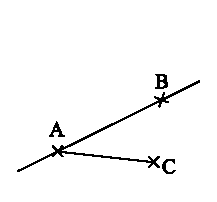
\includegraphics[width=.2\linewidth]{tracerAB-AC} & 
   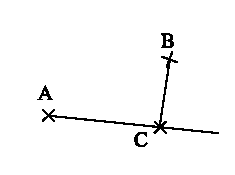
\includegraphics[width=.2\linewidth]{tracerAC-BC} & & 
   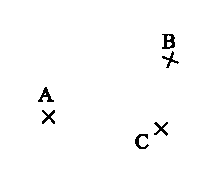
\includegraphics[width=.2\linewidth]{tracerAB-BC-AC}& 
   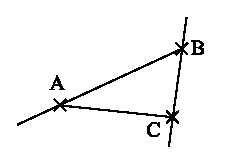
\includegraphics[width=.2\linewidth]{tracer} 					\\ \cline{1-2}\cline{4-5}

   \end{tabular}\\[1em]
  
   \item Lire la consigne de la case \circled{5} et observer la figure correspondant à cette consigne. tracer ensuite la figure de la case \circled{6} et écrire la consigne de la case \circled{7}.
   
   \vspace{1em}
  
   \begin{tabular}{|l|l|l|}
   \hline
    \hfill \circled{5} \hfill			&	\hfill \circled{6} \hfill				&	\hfill \circled{7} \hfill 	\\
    - Tracer la droite passant par 	&	- Tracer le segment 				&					\\
    $E$ et $F$ ;					&	d'extrémités $R$ et $S$ ;			&					\\
    - Tracer le segment 			&	- Tracer la droite passant par 		&					\\
    d'extrémités $E$ et $G$ ;		&	$R$ et $T$ ;					&					\\
    - Tracer la demi-droite 			&	- Tracer la demi-droite 			&					\\
    d'origine $G$ et passant par $F$.	&	d'origine $S$ et passant par $T$.	&					\\ \hline
    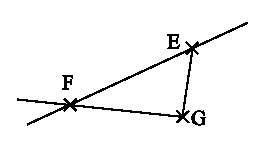
\includegraphics[width=.24\linewidth]{tracerEFG} 			&  
    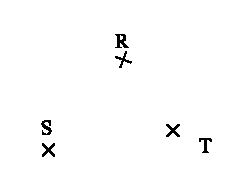
\includegraphics[width=.24\linewidth]{tracerRST}			&
    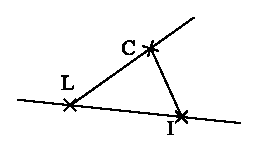
\includegraphics[width=.24\linewidth]{tracerLCI}			\\ \hline
    \end{tabular}\\[1em]
    
   \item Compléter le tableau suivant :
   
   \vspace{1em}
   
   \begin{tabularx}{\linewidth}{|X|X|>{\centering\arraybackslash}X|}
    \hline
    \multicolumn{1}{|c|}{\textbf{Phrase}}	&	\multicolumn{1}{c}{\textbf{Phrase codée}}	&	\multicolumn{1}{|c|}{\textbf{Dessin}}			 	\\  \hline
    								&	Tracer $[UV]$							&	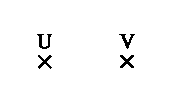
\includegraphics[width=2.6cm]{phraseUV}		\\  \hline
    								&										&	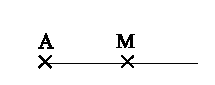
\includegraphics[width=3.2cm]{phraseAM}		\\  \hline
   Tracer la droite passant par $S$ et $T$	&										&	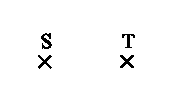
\includegraphics[width=2.6cm]{phraseST}		\\  \hline
   								&										&	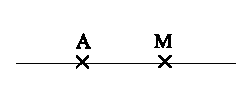
\includegraphics[width=4.0cm]{phraseAM_2}	\\  \hline
   Tracer le segment d'extrémités $M$ et $N$	&									&	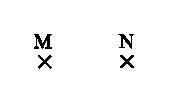
\includegraphics[width=2.6cm]{phraseMN} 	\\  \hline
   								&	Tracer $[KJ)$							&	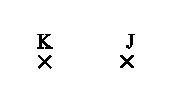
\includegraphics[width=2.6cm]{phraseKJ}		\\  \hline
								&										&	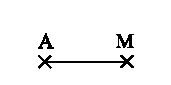
\includegraphics[width=2.6cm]{phraseAM_3}	\\  \hline
   Tracer la demi-droite d'origine $O$ et 	&										&	
\includegraphics[width=2.6cm]{phraseOU}		\\
   passant par $U$					&										&										\\  \hline
   								&	Tracer $(BC)$							&	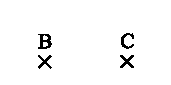
\includegraphics[width=2.6cm]{phraseBC}		\\  \hline
    \end{tabularx}\\[1em]
  
   \end{enumerate} 

  \end{partie}

\end{activite}

%%%%%%%%%%%%%%%%%%%%%%%%%%%%%%%%%%%%%%%%%%%%%

\begin{activite}[Repérer des droites perpendiculaires]

 \begin{minipage}[c]{0.50\linewidth}
  \begin{partie}[Éric a oublié son équerre !]
 
  « Pas de souci, lui dit son professeur, prends une feuille blanche non quadrillée. Tu devrais pouvoir obtenir un angle droit en pliant deux fois cette feuille. »
  
  Réalise une telle équerre.
  
  Qu'obtiens‑tu si tu déplies ta feuille ? 
    \end{partie}
  
  \begin{partie}[Éric utilise sa nouvelle équerre \ldots]
  
  Éric doit replacer l'équerre dans la position qui a permis de construire les droites $d_4$ et $d_7$. \\[0.5em]
  Place l'équerre dans cette position. \\[0.5em]
  Trouve alors un autre couple de droites \textbf{perpendiculaires} sur cette figure en t'aidant de ton équerre.
    \end{partie} \end{minipage} \hfill %
   \begin{minipage}[c]{0.44\linewidth}
   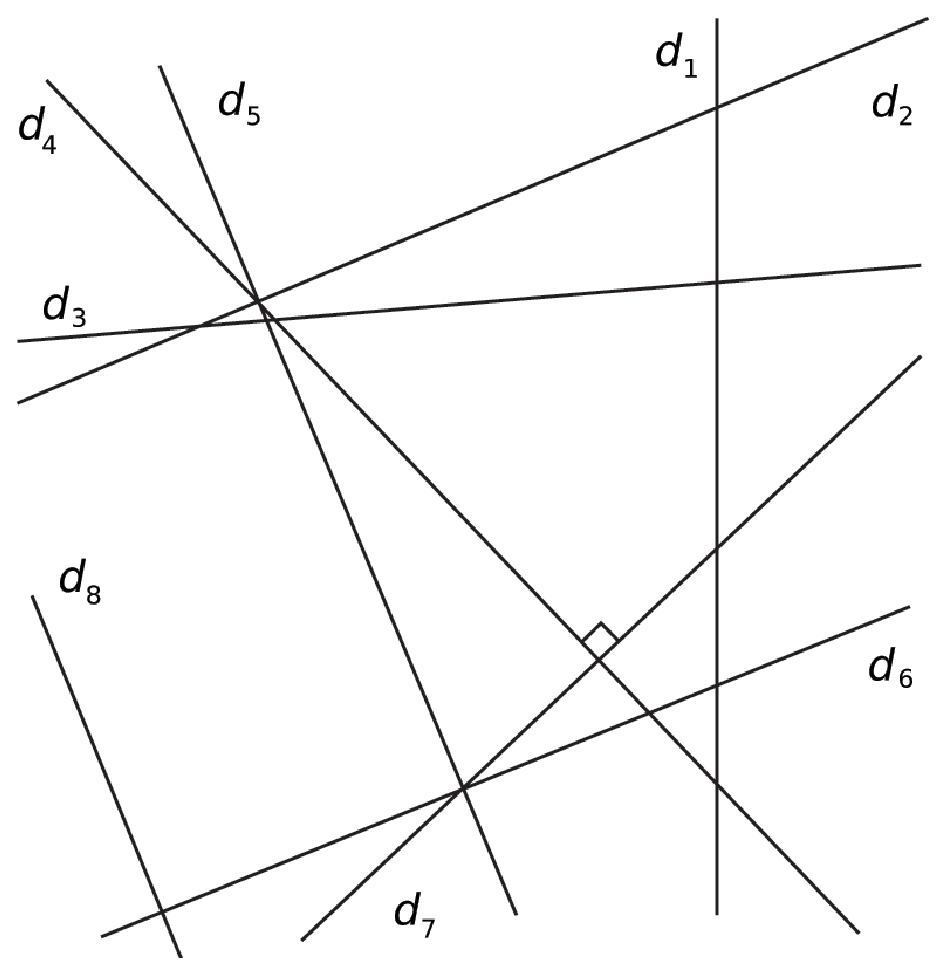
\includegraphics[width=6.1cm]{plusieurs_droites}
   \end{minipage} \\

 \begin{partie}[Utilisation de l'équerre d'Éric]
 
Trace deux droites sécantes $d$ et $d'$. À l'aide de l'équerre que tu as fabriquée, construis une droite perpendiculaire à $d$ et une autre perpendiculaire à $d'$. Tu n'oublieras pas d'ajouter les codages nécessaires.

  \end{partie} 
  
\end{activite}

%%%%%%%%%%%%%%%%%%%%%%%%%%%%%%%%%%%%%%%%%%%%%

\begin{activite}[Droites parallèles]

 \begin{partie}[Deux droites perpendiculaires]
 
  \begin{enumerate}
   \item Place deux points $A$ et $B$.
   \item Trace une droite $d$ ne passant ni par $A$, ni par $B$ et qui coupe $(AB)$.
   \item Trace $d_1$ la perpendiculaire à d passant par $A$, puis la droite $d_2$ perpendiculaire à $d_1$ passant par $B$. Que remarques‑tu ?
   \item Trace $d_3$ la perpendiculaire à $d$ passant par $B$ et $d_4$ la perpendiculaire à $d_3$ passant par $A$. Que peux‑tu dire de $d_2$ et $d_4$ ? Quelles autres remarques du même type peux‑tu faire ? 
   \end{enumerate}
   
  \end{partie} 

 \begin{partie}[Construction à la règle et à l'équerre]
 
 \begin{minipage}[c]{0.66\linewidth}
 La première vignette d'une bande dessinée est représentée ci‑contre. On y a placé une droite $d$ et un point $A$ n'appartenant pas à $d$.
 Complète cette bande dessinée pour expliquer comment, à l'aide de la règle et de l'équerre, tu traces la \textbf{parallèle} à $d$ passant par $A$.
  \end{minipage} \hfill %
 \begin{minipage}[c]{0.3\linewidth}
 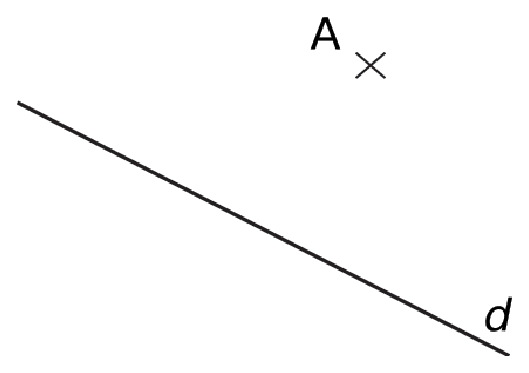
\includegraphics[width=4.2cm]{droiteAd}
  \end{minipage} \\
 
  \end{partie} 

\end{activite}

%%%%%%%%%%%%%%%%%%%%%%%%%%%%%%%%%%%%%%%%%%%%%

\begin{activite}[Tout savoir sur la médiatrice !]

 \begin{partie}[Axes de symétrie d'un segment]
 
 \begin{enumerate}
  \item Sur une feuille blanche, trace un segment $[AB]$.
  \item Plie cette feuille de manière à ce que le point $A$ touche le point $B$, cela fait apparaître un axe de symétrie de ce segment. Le symétrique de $A$ par rapport à cet axe est $B$. Comment s'appelle cet axe ? Repasse‑le en couleur.
  \item Quelles sont ses caractéristiques ?
  \end{enumerate}
  
  \end{partie}
  
 \begin{partie}[Propriété d'un point appartenant à la médiatrice d'un segment]
 
 \begin{enumerate}
  \item Place un point $M$ sur cette médiatrice. Que dire des longueurs $AM$ et $BM$ ?
  \item Que dire alors d'un point qui appartient à la médiatrice d'un segment ?
  \end{enumerate}
  
  \end{partie}
  
 \begin{partie}[Ensemble de points]
 
 \begin{minipage}[c]{0.76\linewidth}
 \begin {enumerate}
  \item Construis un segment $[CD]$ de longueur 5 cm. 
  \item Place $A$, \textbf{équidistant} de $C$ et de $D$. Place trois autres points équidistants de $C$ et de $D$. 
  \item Où semblent se trouver tous les points équidistants de $C$ et $D$ ?
  \item Que dire d'un point équidistant des extrémités d'un segment ?
  \item Déduis‑en une façon de construire la médiatrice d'un segment sans l'équerre. 
  \end{enumerate} 
  \end{minipage} \hfill %
 \begin{minipage}[c]{0.2\linewidth}
 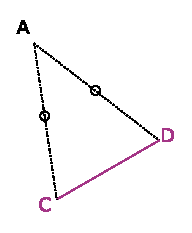
\includegraphics[width=2.8cm]{triangleACD}
  \end{minipage} \\
  
 \end{partie}

\end{activite}

%%%%%%%%%%%%%%%%%%%%%%%%%%%%%%%%%%%%%%%%%%%%%

\begin{activite}[Bissectrice, qui es-tu ?]

 \begin{partie}[Définition] \label{EntDroitSeg_DefBissectrice}

 \begin{minipage}[c]{0.68\linewidth}
 \begin {enumerate}
  \item Sur une feuille blanche, trace un angle $\widehat{ABC}$.
  \item Plie cette feuille de façon à faire apparaître l'axe de symétrie de l'angle. Repasse‑le en couleur. Place un point D sur cet axe (comme sur le croquis ci contre). \label{EntDroitSeg_plier}
  \item Cet axe fait apparaître deux nouveaux angles. Nomme‑les.
  \item Que peut‑on dire de la mesure de ces deux angles ? Justifie. Comment nomme‑t‑on cette droite ?
  \end{enumerate} 
  \end{minipage} \hfill %
 \begin{minipage}[c]{0.26\linewidth}
 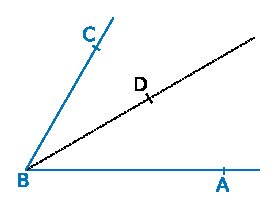
\includegraphics[width=3.8cm]{bissectrice}
  \end{minipage} \\
  
 \end{partie}
 
 \begin{partie}[Construction au compas]
 
 \begin{enumerate}
 \item Construis le point $A'$ symétrique du point $A$ par rapport à la bissectrice de l'angle $\widehat{ABC}$ Tu obtiens ce point en reportant le point A sur la droite $[BC)$ en pliant la feuille comme au point \ref{EntDroitSeg_plier} de la partie \ref{EntDroitSeg_DefBissectrice}. Que dire des longueurs $BA$ et $BA'$ ?
 \item Que représente la bissectrice de l'angle $\widehat{ABC}$ pour le segment $[AA']$ ?
 \item Déduis‑en une façon de construire la bissectrice d'un angle sans rapporteur.
  \end{enumerate}              
  \end{partie}
 
\end{activite}

%%%%%%%%%%%%%%%%%%%%%%%%%%%%%%%%%%%%%%%%%%%%%

\begin{activite}[De qui est-ce la trace ?]

 \begin{partie}
 Sur ton cahier, place un point $O$. Recherche tous les points situés à 3 cm du point $O$. 
  \end{partie}

 \begin{partie}
 \begin{minipage}[c]{0.78\linewidth}
 Un système d'arrosage automatique est formé d'un jet qui arrose dans toutes les directions jusqu'à 4 m.
  \begin {enumerate}
  \item Représente sur ton cahier la zone arrosée par le jet en appelant $J$ l'emplacement du jet. (1 cm représentera 1 m.)
  \item Comment peux‑tu définir les points de la zone arrosée ? 
  \end{enumerate} 
  \end{minipage} \hfill %
 \begin{minipage}[c]{0.16\linewidth}
 
\includegraphics[width=2cm]{arrosage}
  \end{minipage} \\
    
  \end{partie}

\end{activite}

%%%%%%%%%%%%%%%%%%%%%%%%%%%%%%%%%%%%%%%%%%%%%

\begin{activite}[Des constructions]

 \begin{partie}[Du programme à la figure]
 Réalise la suite d'instructions suivantes :
 \begin{itemize}
  \item Trace un cercle $(\mathcal{C})$ de centre $O$ et de rayon 5 cm.
  \item Place, sur le cercle, deux points $A$ et $B$ \textbf{diamétralement opposés}.
  \item Construis le cercle $(\mathcal{C}_1)$ de diamètre $[OA]$ et le cercle $(\mathcal{C}_2)$ de diamètre $[OB]$.
  \item Trace le cercle $(\mathcal{C}_3)$ de centre $A$ passant par $O$.
  \item Nomme $E$ et $F$ les \textbf{points d'intersection} des cercles $(\mathcal{C})$ et $(\mathcal{C}_3)$.
  \item Trace le cercle $(\mathcal{C}_4)$ de centre $B$ et de rayon $OB$.
  \item Les cercles $(\mathcal{C})$ et $(\mathcal{C}_4)$ se coupent en $G$ et $H$.
  \end{itemize}
  
  \end{partie}
  
 \begin{partie}[De la figure au programme]
 \begin{minipage}[c]{0.48\linewidth} 
Construis la figure ci‑contre donnée 

par son croquis.

Écris le programme de construction.
 \end{minipage} \hfill %
 \begin{minipage}[c]{0.46\linewidth}
 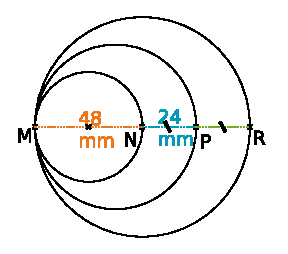
\includegraphics[width=4.2cm]{figure-programme}
  \end{minipage} \\
  
  \end{partie}

\end{activite}

%%%%%%%%%%%%%%%%%%%%%%%%%%%%%%%%%%%%%%%%%%%%%
